\subsection{Trace} \label{trace}
Um den Ablauf innerhalb der Software nachvollziehen zu können wird nachfolgend die Sogenannte "Trace" beim Aufstarten der Software und beim Auslösen eines Ereignisses aufgezeigt. Die "Trace" wird innerhalb der Software mithilfe der Klasse traceV4 in die Konsole ausgegeben.

\paragraph{Trace beim Aufstarten}
 
 \begin{figure}[H]
	\centering
	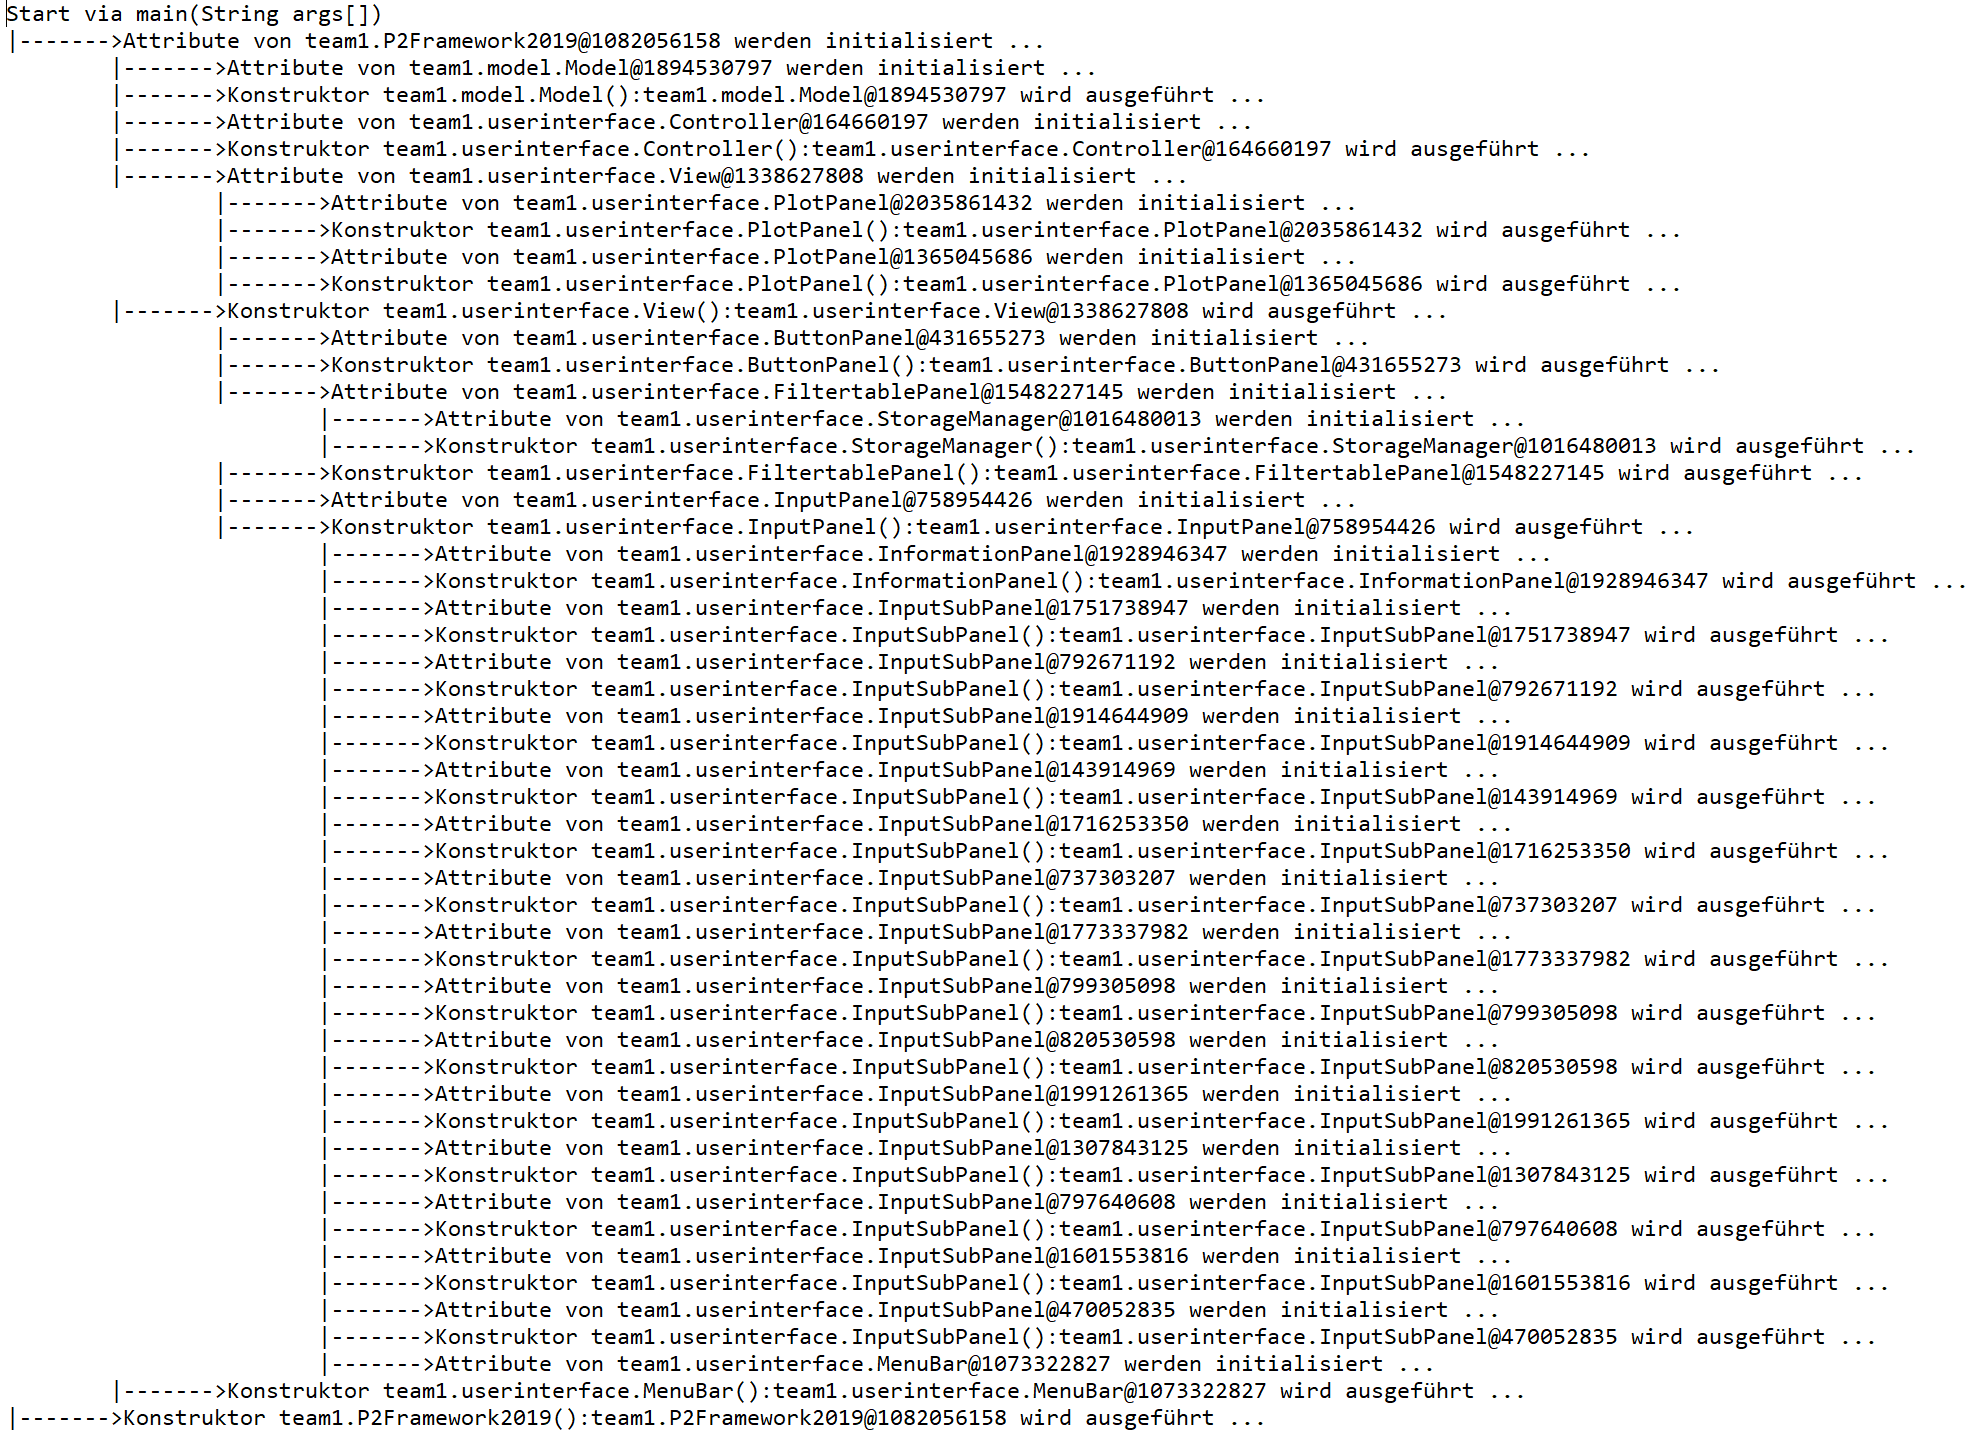
\includegraphics[width=16cm]{trace_start.png}
	\caption{Trace beim Aufstarten}
	\label{fig:tracestart}
\end{figure} 

\newpage

\paragraph{Trace bei einem Event}

\begin{figure}[H]
	\centering
	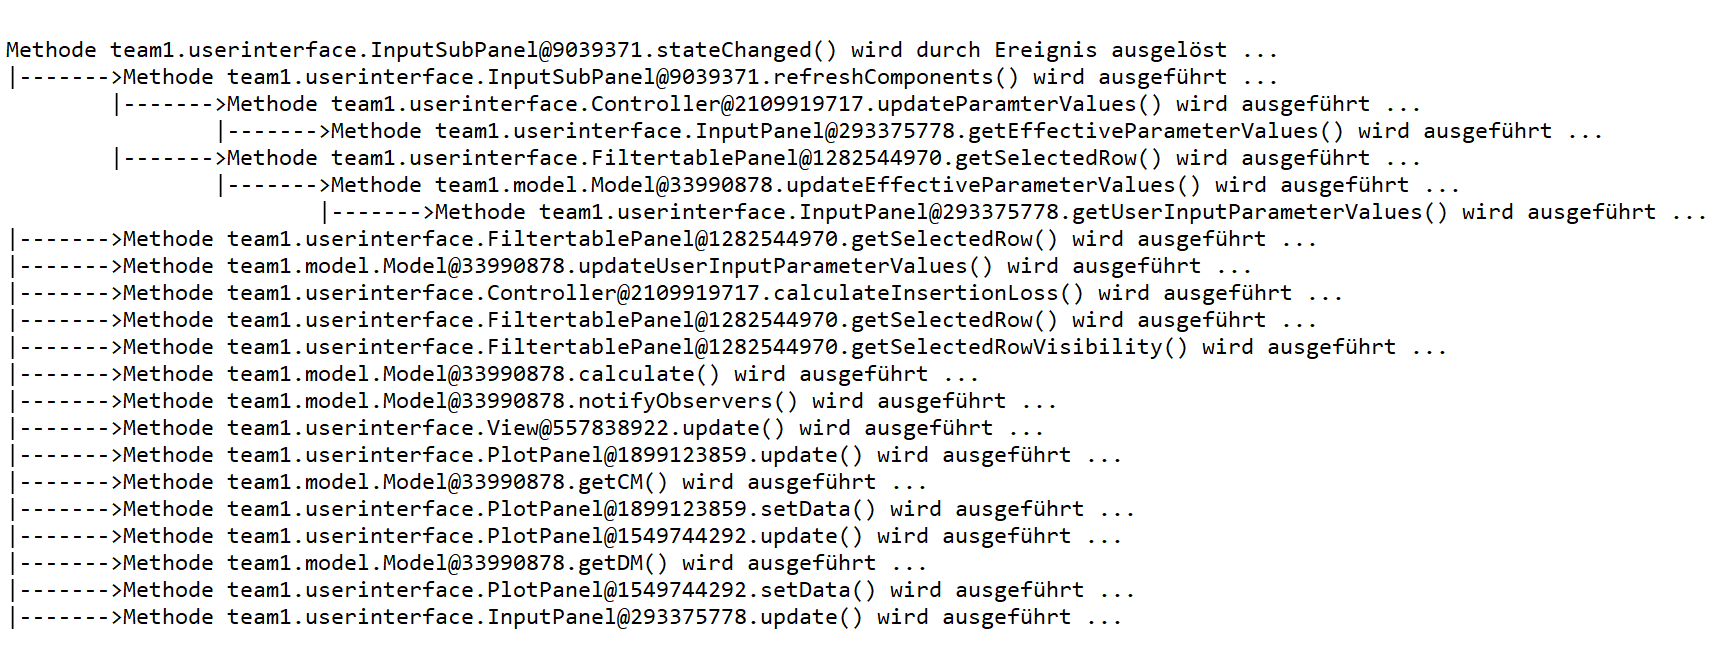
\includegraphics[width=16cm]{trace_event.png}
	\caption{Trace beim event}
	\label{fig:traceevent}
\end{figure} 

\newpage